\documentclass[tikz,border=4mm]{standalone}
      \usepackage{tikz}
      \usetikzlibrary{arrows.meta,positioning,calc,shapes.geometric}
      \begin{document}
      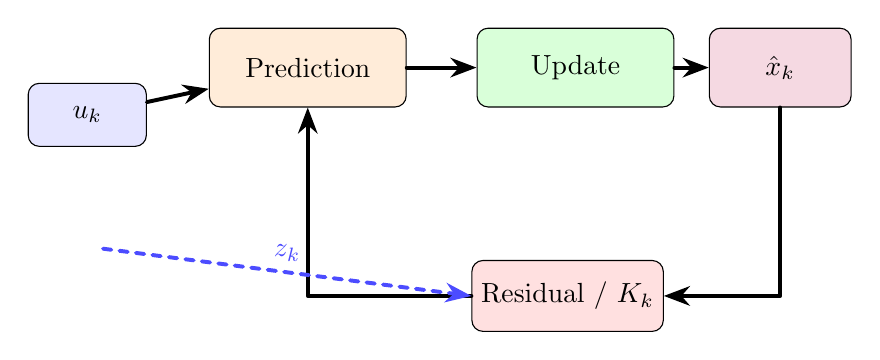
\begin{tikzpicture}[>=Stealth, line cap=round, line join=round]

\node[draw, rounded corners, fill=blue!10, minimum width=1.5cm, minimum height=0.8cm] (u) at (1.4,4.5) {$u_k$};
\node[draw, rounded corners, fill=orange!15, minimum width=2.5cm, minimum height=1cm] (pred) at (4.2,5.1) {Prediction};
\node[draw, rounded corners, fill=green!15, minimum width=2.5cm, minimum height=1cm] (upd) at (7.6,5.1) {Update};
\node[draw, rounded corners, fill=purple!15, minimum width=1.8cm, minimum height=1cm] (state) at (10.2,5.1) {$\hat{x}_k$};
\node[draw, rounded corners, fill=red!12, minimum width=2.2cm, minimum height=0.9cm] (gain) at (7.5,2.2) {Residual / $K_k$};
\draw[->, line width=0.05cm] (u) -- (pred);
\draw[->, line width=0.05cm] (pred) -- (upd);
\draw[->, line width=0.05cm] (upd) -- (state);
\draw[->, line width=0.05cm] (state.south) |- (gain.east);
\draw[->, line width=0.05cm] (gain.west) -| (pred.south);
\draw[->, line width=0.05cm, dashed, blue!70] (1.6,2.8) -- node[above] {$z_k$} (gain.west);

      \end{tikzpicture}
      \end{document}
